%!TEX program = xelatex
\documentclass[11pt,class=book]{standalone}
%\usepackage[utf8]{inputenc}
\usepackage[french]{babel}
\usepackage[french]{translator}
\usepackage[T1]{fontenc}
\usepackage{fontspec}
\usepackage[table,svgnames]{xcolor}

\usepackage{pgf}
\usepackage{tikz}

\usepackage{array}
\usepackage{tabularx}
\usepackage{multirow}
\usepackage{pgf-umlsd}
\usepackage{pgfgantt}

\usetikzlibrary{shapes}
\usetikzlibrary{arrows.meta}
\usetikzlibrary{calc}

\definecolor{bg_color}{RGB}{250,250,229}

\colorlet{color1}{cyan!50}
\colorlet{color2}{red!30!green!40}
\colorlet{color3}{orange!50}
\colorlet{color4}{violet!60!blue!55}

\newganttlinktype{bartobardown}{
	\ganttsetstartanchor{south east}
	\ganttsetendanchor{north west}
	\draw [/pgfgantt/link] (\xLeft, \yUpper) -- (\xRight, \yLower);
}
\newganttlinktype{bartobarup}{
	\ganttsetstartanchor{north east}
	\ganttsetendanchor{south west}
	\draw [/pgfgantt/link] (\xLeft, \yUpper) -- (\xRight, \yLower);
}
\newganttlinktype{milestonetobardown}{
	\ganttsetstartanchor{south}
	\ganttsetendanchor{north west}
	\draw [/pgfgantt/link] (\xLeft, \yUpper) -- (\xRight, \yLower);
}
\newganttlinktype{bartomilestonedown}{
	\ganttsetstartanchor{south east}
	\ganttsetendanchor{north}
	\draw [/pgfgantt/link] (\xLeft, \yUpper) -- (\xRight, \yLower);
}


\begin{document}
	\begin{tikzpicture}[x=1pt,y=1pt,inner sep=0pt,outer sep=0pt]
		\tikzset{block/.style={
			draw,
			rectangle,
			minimum width=100,
			minimum height=280,
			fill=gray!70,
		}}
		\tikzset{blocktext/.style={
			align=center,
			text width=100pt,
			align=center,
		}}
		\tikzset{subdga/.style={
			draw,
			rectangle,
			minimum width=240pt,
			text width=240pt,
			minimum height=30pt,
			align=center,
			yshift=-14pt,
			fill=gray!40,
		}}

		%---------------------------------
		% Ministère des Armées
		\node[
			draw,
			rectangle,
			minimum width=460,
			minimum height=300,
			fill=gray,
			anchor=north west,
		] (main) at (0,0) {};
		\node[
			blocktext,
			anchor=west,
		] (minarm) at (main.west) {
\includegraphics[width=80pt]{logos/Ministere_des_Armees}};

		%---------------------------------
		% DGA
		\node[
			block,
			anchor=west
		] (dgablock) at (minarm.east) {};
		\node[
			blocktext,
			anchor=west,
		] (dga) at (dgablock.west) {
\includegraphics[width=80pt]{logos/DGA}};

		%---------------------------------
		% EMA
		\node[
			block,
			anchor=west,
			xshift=20pt,
		] (emablock) at (dgablock.east) {};
		\node[
			blocktext,
			anchor=west,
		] (ema) at (emablock.west) {%
			
\includegraphics[width=65pt]{logos/DRM}\\[10pt]
			
\includegraphics[width=65pt]{logos/Service_de_sante_des_armees}\\[10pt]
			\Huge\ldots%
		};

		%---------------------------------
		% EMA
		\node[
			block,
			anchor=west,
			xshift=20pt,
		] (emablock) at (dgablock.east) {};
		\node[
			blocktext,
			anchor=west,
		] (ema) at (emablock.west) {
\includegraphics[width=80pt]{logos/Etat_Major_des_armees}};

		%---------------------------------
		% DGRIS
		\node[
			block,
			anchor=west,
			xshift=20pt,
		] (etcblock) at (emablock.east) {};
		\node[
			blocktext,
			anchor=west,
		] (etc) at (etcblock.west) {%
			
\includegraphics[width=80pt]{logos/DGSE}\\[10pt]
			
\includegraphics[width=80pt]{logos/DGRIS}\\[10pt]
			\Huge\ldots%
		};

		%---------------------------------
		% DGA
		\node[
			block,
			minimum width=350,
			anchor=west
		] (dgablock) at (minarm.east) {};
		\node[
			blocktext,
			anchor=west,
		] (dga) at (dgablock.west) {
\includegraphics[width=80pt]{logos/DGA}};

		%---------------------------------
		% sub DGA
		\node[
			subdga,
			anchor=north west,
			xshift=100pt,
		] (subdga) at (dgablock.north west) {Direction Technique};
		\node[
			subdga,
			anchor=north west,
		] (subdga) at (subdga.south west) {Direction du Développement International};
		\node[
			subdga,
			anchor=north west,
		] (subdga) at (subdga.south west) {Direction des opérations};
		\node[
			subdga,
			anchor=north west,
		] (subdga) at (subdga.south west) {Direction de la Stratégie};
		\node[
			subdga,
			anchor=north west,
		] (subdga) at (subdga.south west) {Direction des Plans, des Programmes, et du Budget};
		\node[
			subdga,
			anchor=north west,
		] (subdga) at (subdga.south west) {Services de soutien};

		%---------------------------------
		% Direction Technique
		\node[
			draw,
			rectangle,
			minimum width=240pt,
			minimum height=250pt,
			fill=gray!40,
			anchor=north west,
			xshift=100pt,
			yshift=-14pt,
		] (subdga) at (dgablock.north west) {};
		\node[
			text width=240pt,
			minimum height=30pt,
			align=center,
			anchor=north,
		] (subdga) at (subdga.north) {Direction Technique};
		\node[
			text width=240pt,
			align=center,
			yshift=-40pt,
			anchor=north west,
			xshift=100pt,
		] (subdga) at (dgablock.north west) {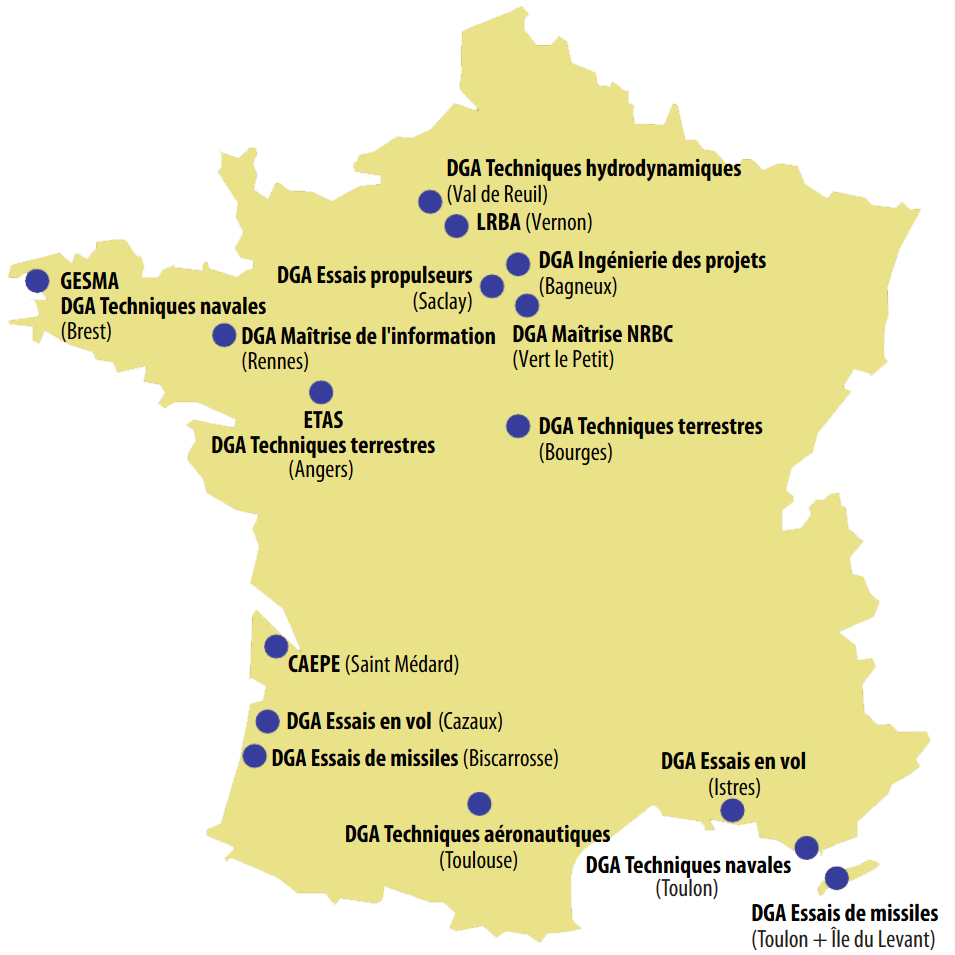
\includegraphics[width=220pt]{Carte_centres_expertise_et_essais_DGA}};
		\node[
			text width=240pt,
			align=center,
			yshift=-40pt,
			anchor=north west,
			xshift=100pt,
		] (subdga) at (dgablock.north west) {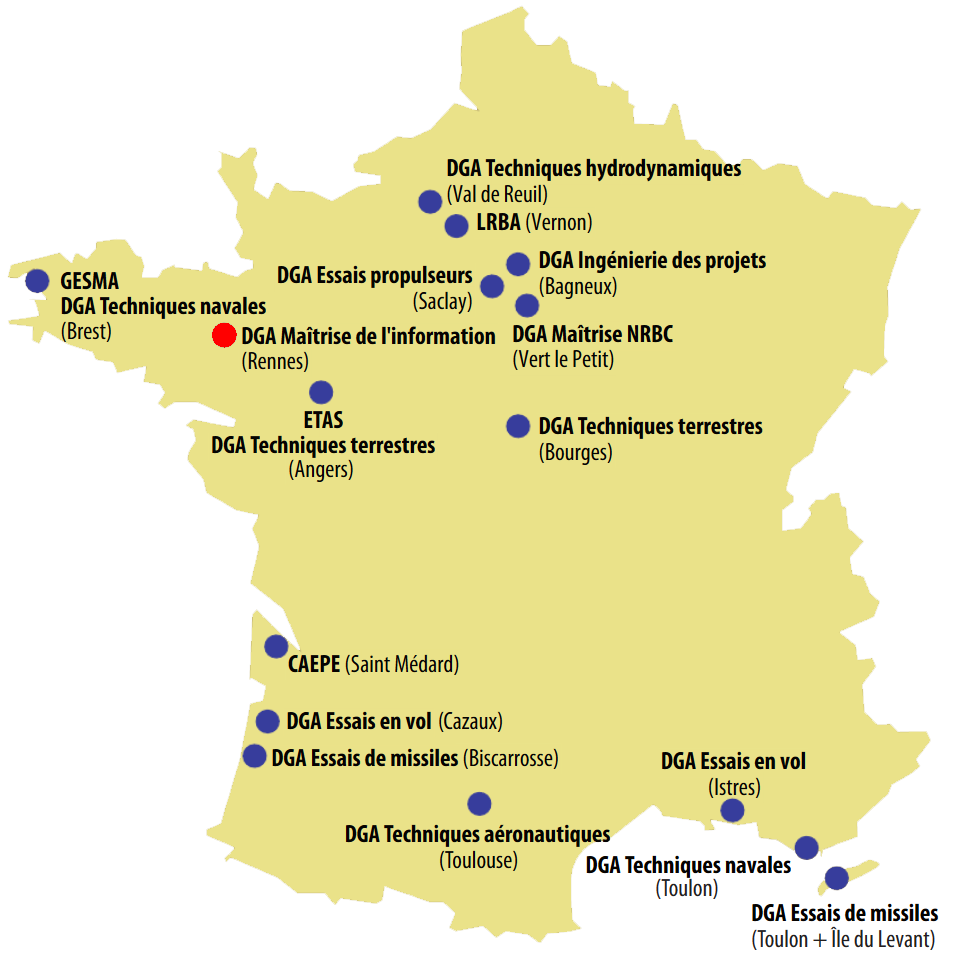
\includegraphics[width=220pt]{Carte_centres_expertise_et_essais_DGA_MI}};
	\end{tikzpicture}
\end{document}
